\documentclass[12pt,letterpaper]{article}

\usepackage[letterpaper, margin=1in]{geometry}
\usepackage[utf8]{inputenc} % OJO!!!  => MANTENER ESTA LINEA PARA FACIL CONVERSION A WORD EN EL FUTURO ...
% \usepackage[spanish]{babel}
\usepackage{graphicx} 
\usepackage{array}
\usepackage{tabularx}
\usepackage{amssymb, amsmath}

% Paquetes extras ... 
\usepackage{subfigure}
\usepackage{color}
\definecolor{mygreen}{RGB}{28,172,0} % color values Red, Green, Blue
\definecolor{mylilas}{RGB}{170,55,241}

\usepackage{hyperref}
\usepackage{enumitem}

\usepackage{amsmath,amsfonts,amssymb,amsthm,cancel,icomma,nicefrac,mathrsfs,
            eurosym,verbatim,environ,ifthen,ifdraft,pdfpages,float,booktabs}
\allowdisplaybreaks[1] 

\usepackage{color}
\definecolor{lstgrey}{rgb}{0.95,0.95,0.95}
\usepackage{listings}
\lstset{language=Matlab,
       backgroundcolor=\color{lstgrey},
       frame=single,
       basicstyle=\footnotesize\ttfamily,
       captionpos=b,
       tabsize=2,
  }

\lstset{language=Matlab,%
  %basicstyle=\color{red},
  breaklines=true,%
  morekeywords={matlab2tikz},
  keywordstyle=\color{blue},%
  morekeywords=[2]{1}, keywordstyle=[2]{\color{black}},
  identifierstyle=\color{black},%
  stringstyle=\color{mylilas},
  commentstyle=\color{mygreen},%
  showstringspaces=false,%without this there will be a symbol in the places where there is a space
  numbers=left,%
  numberstyle={\tiny \color{black}},% size of the numbers
  numbersep=9pt, % this defines how far the numbers are from the text
  emph=[1]{for,end,break},emphstyle=[1]\color{red}, %some words to emphasise
  %emph=[2]{word1,word2}, emphstyle=[2]{style},    
}


\title{Homework 3 - Monte Carlo Analysis}
\author{Jose Eduardo Laruta Espejo \\ Facultad de Ingeniería - Universidad Mayor de San Andrés}
\begin{document}
\maketitle

\section{Projectile model}
We are going to use the following model for our projectile:

\begin{equation}
    \sum{F} = M a
\end{equation}

If we take the $x$ and $y$ components and the gravity effect into account we have:

\begin{align}
    M a_x &= -F_x \\ 
    M a_y &= -F_y - F_g \\ 
    F_x &= F\cos{\theta_0} \\
    F_y &= F\sin{\theta_0} \\
    F &= Bv + D|v|^2
\end{align}

our states are given by:

\begin{align*}
    x_1 &= y &x_2&=v_y &x_3&=x &x_4&=v_x\\
\end{align*}

then, our state space form model is as follows:

\begin{align}
    \dot{x_1} &= x_2 \\
    \dot{x_2} &= -\frac{(Bv + D|v|^2)cos(\theta_0)}{M} - g \\
    \dot{x_3} &= x_4 \\
    \dot{x_4} &= -\frac{(Bv + D|v|^2)sin(\theta_0)}{M}
\end{align}

where $v = \sqrt{x_2^2 + x_4^2}$ the current magnitude of the velocity and $\theta_0$ the initial angle. The initial conditions are 
defined statistically by $E[\theta_0] = 45[deg]$ , $E[v_0]=200[m/s]$ and standard deviation of 3\%. Then, the initial condition vector 
given $\theta_0$ and $v_0$ are:

\begin{equation*}
    x_0 = \begin{bmatrix}
        0 \\
        v_0 \sin{\theta_0} \\
        0 \\
        v_0 \cos{\theta_0}
    \end{bmatrix}
\end{equation*}

the model expressed in matlab code:
\lstinputlisting[label=lst:model]{../matlab/projectile_model.m}

\section{Monte Carlo Simulation}
The code for the Simulation is as follows:
\lstinputlisting[label=lst:simu]{../matlab/run_projectile.m}
after running the simulation the resulting plots are:

%%%% Figura 1 %%%%%%
\begin{figure}[!h] 
    \centering
    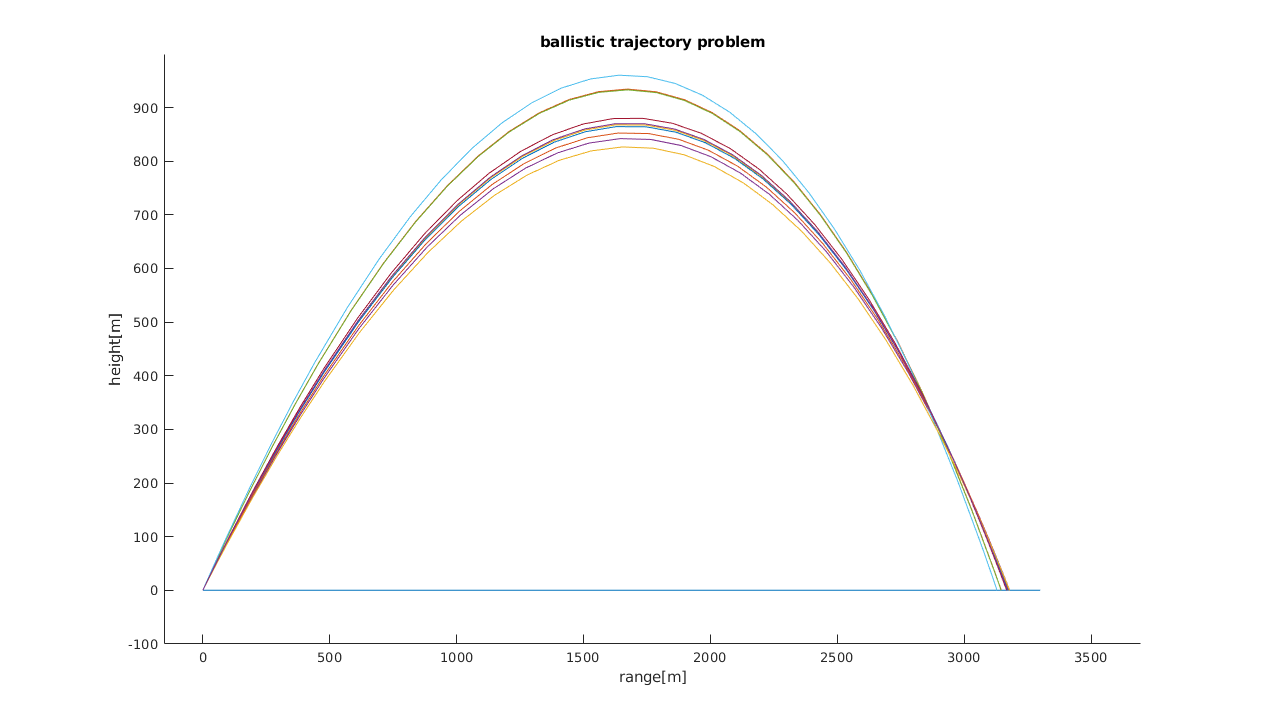
\includegraphics[width=0.9\textwidth]{../matlab/img/simu.png}
    \caption{Simulation of the model}
    \label{fig:simu}
    \end{figure}
    
    In the case of the simulation of the projectile trajectories, Fig \ref{fig:simu} shows clearly the variation due to random
    initial conditions.
    
    For the statistics we can se clearly the convergence of the mean as soon as the Monte Carlo trials begin to 
    increase, the same for the standard deviation. In Fig \ref{fig:mean} the mean is slowly converging and the interval of confidence
    decrease in size. The same goes for Sigma in Fig \ref{fig:sigma}. Just for fun, the plots for 10000 iteration are shown in Figs \ref{fig:mean10}
    and \ref{fig:sigma10}, were we can see the convergence of the mean in 3159 m and sigma in 19.62 m.
    %%%% Figura 1 %%%%%%
    \begin{figure}[!h] 
        \centering
        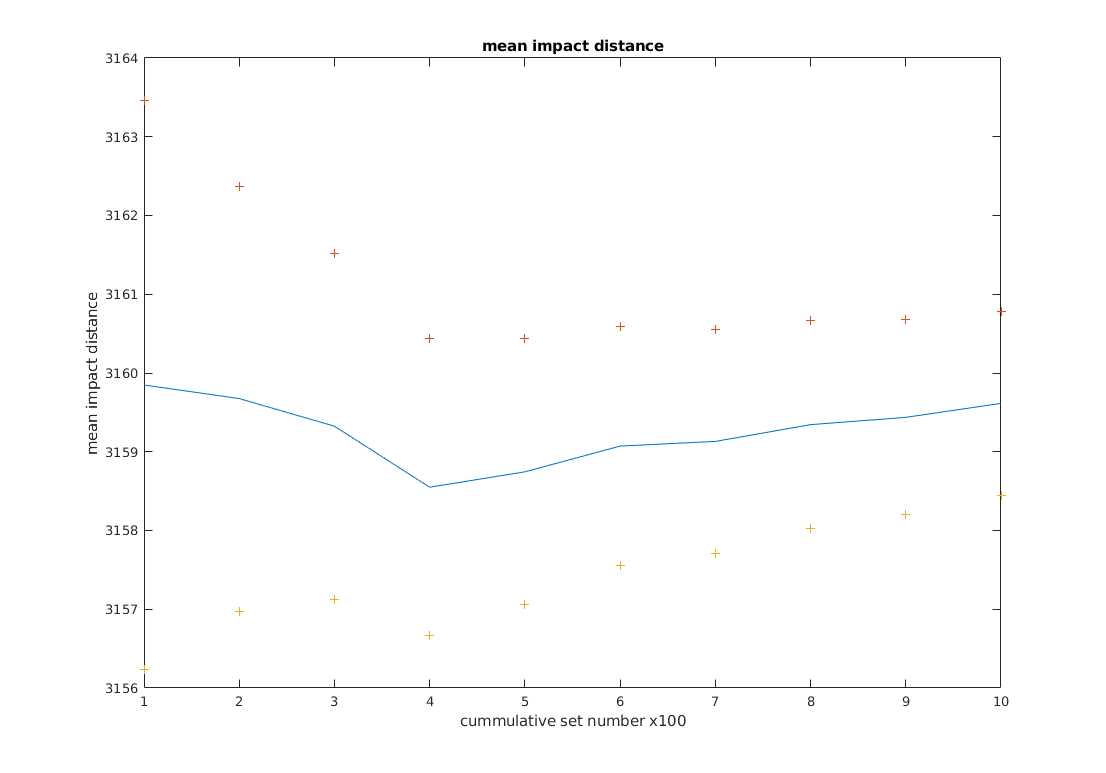
\includegraphics[width=0.8\textwidth]{../matlab/img/mean.png}
        \caption{Mean convergence 1000 runs}
        \label{fig:mean}
    \end{figure}
    
    %%%% Figura 1 %%%%%%
    \begin{figure}[!h] 
        \centering
        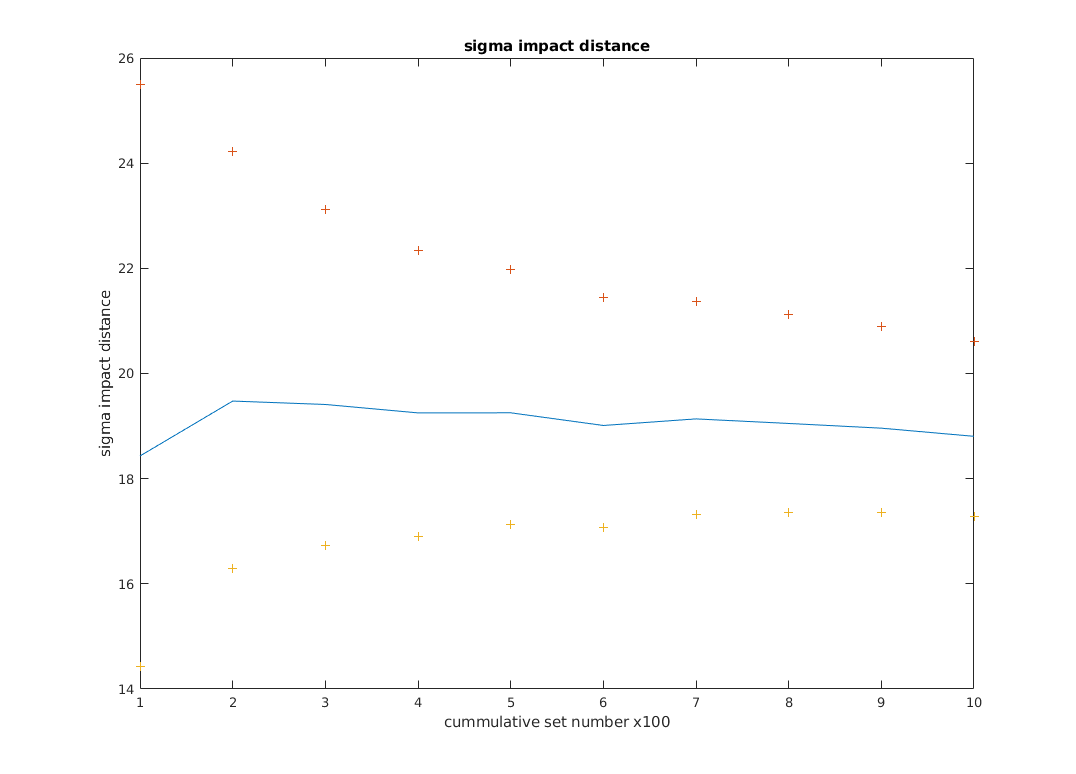
\includegraphics[width=0.8\textwidth]{../matlab/img/sigma.png}
        \caption{Sigma convergence 1000 runs}
        \label{fig:sigma}
    \end{figure}

    %%%% Figura 1 %%%%%%
    \begin{figure}[!h] 
        \centering
        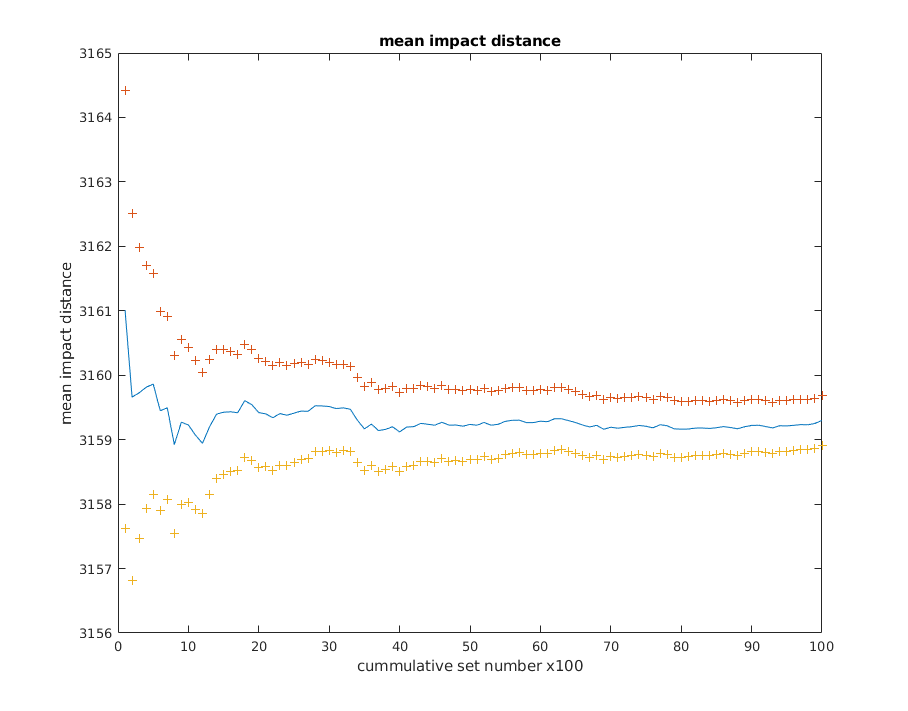
\includegraphics[width=0.8\textwidth]{../matlab/img/mean10.png}
        \caption{Mean convergence 10000 runs}
        \label{fig:mean10}
    \end{figure}
    
    %%%% Figura 1 %%%%%%
    \begin{figure}[!h] 
        \centering
        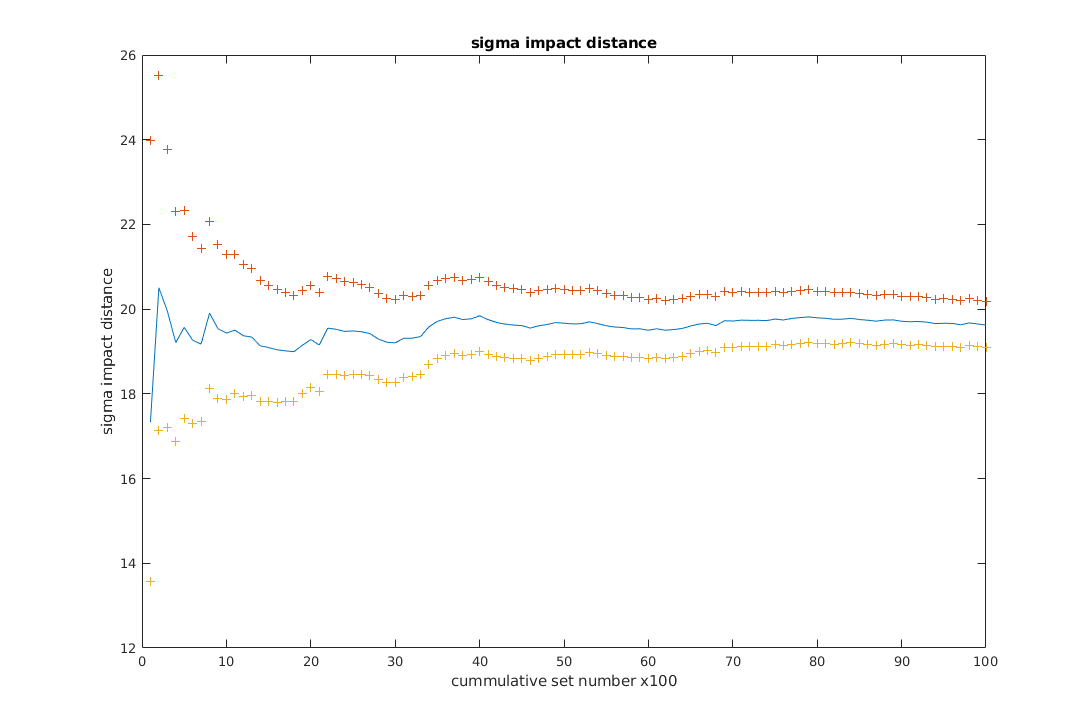
\includegraphics[width=0.8\textwidth]{../matlab/img/sigma10.png}
        \caption{Sigma convergence 10000 runs}
        \label{fig:sigma10}
    \end{figure}
\end{document}